\documentclass[../Mathe_Aufgaben.tex]{subfiles}
\begin{document}
	\chapter{Differentialrechnung - Teil 2}
	\chapter{Integralrechnung - Teil 2}	
	\chapter{Kurvendiskussion - Teil 2}

	\section{Wurzelfunktionen}
	\label{sec:aufg-wurzel}

	\begin{komplexaufgaben}{sec:aufg-wurzel}
		\komplexaufgabe{Gegeben sei die Funktion $f(x)=x\sqrt{6-x}$.}{
			\item Geben Sie den Definitionsbereich von $f$ an.
			\item Bestimmen Sie $f'$ und $f''$.
			\item Untersuchen Sie $f$ auf Nullstellen und Extrema.
			\item Zeichnen Sie den Graphen von $f$ im Bereich $-1 \le x \le 6$.
			\item Bestimmen Sie die Gleichung der Tangente an den Graphen von $f$ im Punkt $P(0\mid f(0))$.
		}

		\komplexaufgabe{Gegeben sei die Funktion $f(x)=x\sqrt{4-x^2}$.}{
			\item Geben Sie den Definitionsbereich von $f$ an und bestimmen Sie die Nullstellen.
			\item Untersuchen Sie $f$ auf Extrema und Wendepunkte.
			\item Zeichnen Sie den Graphen von $f$.
			\item Geben Sie die Gleichung der Wendetangente an.
			\item Untersuchen Sie das Verhalten von $f'$ für $x \to 2$ und $x \to -2$.
		}

		\komplexaufgabe{(MMS) Gegeben sind die Funktionen $f(x)=2\sqrt{x}$ und die Funktionenschar $g_t(x)=2t\sqrt{t^2+1-x}$.}{
			\item Skizzieren Sie die Graphen von $f$, $g_1$ und $g_2$. Bestimmen Sie dazu den Definitionsbereich und die Nullstelle von $g_1$ und $g_2$.
			\item Bestimmen Sie den Schnittpunkt $S_1$ der Graphen von $f$ und $g_1$ und entsprechend den Schnittpunkt $S_2$ von $f$ und $g_2$.
			\item Berechnen Sie den allgemeinen Schnittpunkt $S_t$ der Graphen von $f$ und $g_t$.
			\item Weisen Sie rechnerisch nach: Die Graphen von $f$ und $g_t$ schneiden sich in $S_t$ \textit{orthogonal} (rechtwinklig).
		}
	\end{komplexaufgaben}

	\begin{loesungssektion}{sec:aufg-wurzel}
		\setcounter{exo}{0}
		\begin{komplexloesungen}{sec:aufg-wurzel}
			\komplexloesung{}{
				\item $D_f=(-\infty,6]$
				\item $f'(x)=\frac{3(4-x)}{2\sqrt{6-x}}$; $f''(x)=\frac{3(x-8)}{4(6-x)^{3/2}}$ (für $x<6$)
				\item Nullstellen: $x_1=0$, $x_2=6$. Maximum bei $x=4$: $f(4)=4\sqrt{2}$.
				\item Skizze: $f(-1)=-\sqrt{7}$, $f(0)=0$, $f(4)=4\sqrt{2}$, $f(6)=0$.
				\item Tangente in $P(0\mid 0)$: $f'(0)=\sqrt{6}$; $y=\sqrt{6}\,x$.
			}

			\komplexloesung{}{
				\item $D_f=[-2,2]$; Nullstellen: $x=0$, $x=\pm 2$.
				\item Extrema: $f'(x)=\frac{4-2x^2}{\sqrt{4-x^2}}=0 \Rightarrow x=\pm\sqrt{2}$; Max. bei $x=\sqrt{2}$, Min. bei $x=-\sqrt{2}$. Wendepunkte: $f''=0 \Rightarrow x=0$ (Wendepunkt $(0|0)$).
				\item (Skizze)
				\item Wendetangente in $(0|0)$: $f'(0)=2$; $y=2x$.
				\item $f'(x)=\frac{4-2x^2}{\sqrt{4-x^2}} \to -\infty$ für $x\to\pm2$ (senkrechte Tangente an den Rändern).
			}

			\komplexloesung{}{
				\item $D_{g_t}=(-\infty,\,t^2+1]$; Nullstelle: $x=t^2+1$. (Skizzen für $t=1$: $g_1(x)=2\sqrt{2-x}$, Nullstelle $x=2$; für $t=2$: $g_2(x)=4\sqrt{5-x}$, Nullstelle $x=5$.)
				\item $f(x)=g_1(x) \Rightarrow 2\sqrt{x}=2\sqrt{2-x} \Rightarrow x=1$; $S_1=(1,2)$. $S_2=(4,4)$.
				\item $2\sqrt{x}=2t\sqrt{t^2+1-x} \Rightarrow x=t^2(t^2+1-x) \Rightarrow x=\frac{t^2(t^2+1)}{t^2+1}=t^2$; $S_t=(t^2,\,2t)$.
				\item $f'(t^2)=\frac{1}{t}$; $g_t'(t^2)=-t$. Produkt der Steigungen: $\frac{1}{t}\cdot(-t)=-1$ $\Rightarrow$ senkrechter Schnitt.
			}
		\end{komplexloesungen}
	\end{loesungssektion}

	\section{Exponential- und Logarithmusfunktionen}
	\label{sec:exp-log}
	\subsection{Grundlegende Aufgabentypen Exponentialfunktionen} 
	\label{sec:grundlegendAufgExp}
	
	
	\begin{kurzaufgaben}{sec:grundlegendAufgExp}
		
			\kurzaufgabe[3]{Bestimmen Sie die Lösungen der Exponentialgleichungen.}{
				\item \(e^{2x+1}-1=1\)
				\item \(3e^{x}=e^{-x}\)
				\item \(4e^{x}=e^{2x}\)
				\item \(e^{x+1}=e^{-x}\)
				\item \(5e^{2x}=3e^{3x}\)
				\item \(2e^{-0.5x}=7e^{-2x}\)
				\item \(4e^{x}+2=6e^{-x}\)
				\item \(2e^{x}-2=12e^{-x}\)
			}

			\kurzaufgabe[2]{Bestimmen Sie die Schnittpunkte der Funktionsgraphen von $f$ und $g$. }{
				\item \(f(x)=2.5\cdot e^{x}\), $g(x)=e^{2\cdot x}$
				\item \(f(x)=x\cdot e^{x+1}\), $g(x)=x$
			}
	\end{kurzaufgaben}

	\begin{komplexaufgaben}{sec:grundlegendAufgExp}

			\komplexaufgabe{Die Funktion $f(x)=axe^{bx}$ hat im Punkt $P(2|e^{-2})$ ihren 
			Funktionswert als Steigung. Bestimmen Sie $a$ und $b$.} {}

			\komplexaufgabe{Wie muss $a$ gewählt werden, damit die Graphen von 
			$f(x)=e^x$ und $g(x)=ax^3$ sich \textit{berühren}? Berechnen Sie auch den Berührungspunkt.}{}	

			\komplexaufgabe{Wie sind $a$ und $b$ zu wählen, damit sich die Graphen von $f(x)=e^x$ und $g(x)=e^{ax+b}$
			 bei $x=1$ \textit{senkrecht} schneiden?} {}

			\komplexaufgabe{Gegeben sei die Funktion $f(x)=(2x+3)\cdot e^{-x}$. Ermitteln Sie,  unter welchem Winkel $\alpha$
			die Tangente an den Graphen an der Stelle $x=-1$ die $x$-Achse schneidet.} {}

			\komplexaufgabe{Gegeben seien die Funktionen $f(x)=e^x$ und $g(x)=e^{-x+2}$.Ermitteln Sie
			 unter welchem Winkel $\gamma$ sich die Graphen von $f$ und $g$ schneiden.} {}

			\komplexaufgabe{Ermitteln Sie, welche Ursprungsgerade $g$ ist Tangente an den Graphen von 
			$f(x)=e^{0.5x}$.}{} 

			\komplexaufgabe{Ermitteln Sie die Gleichung der Tangente an den Graphen der Funktion $f(x)=e^{-x}$
			die parallel zur Sehne durch die beiden Punkte $P(-1|e)$ und $Q(1|\frac{1}{e})$ des graphen von $f$ ist.}{}

			\komplexaufgabe{Die Graphen von $f(x)=e^x$ und $g(x)=e^{0.5x}$ besitzen nur an einer Stelle $x$ den gleichen
			Anstieg. Ermitteln Sie diese Stelle und geben Sie die Tangente von $f$ und die Normale von $g$ an dieser Stelle an.}{}
			
			\komplexaufgabe{Gegeben sind die Funktionen $f(x)=4-x$ und $g(x)= 4\cdot e^{-x}$. Ermitteln Sie die Stelle
			des Intervalls $\left[0,2\right]$ an der die Differenz der Funktionswerte maximal wird.}{}

			\komplexaufgabe{Gegeben seien die Funktionen $f(x)=e^{-x}$ und $g(x)=2\cdot e^{0.5x}$. Die Gerade $y=k,k>0$ schneidet die 
			Graphen der Funktionen $f$ und $g$. Diese Schnittpunkte markieren die oberen Eckpunkte eines achsenparallen Rechtecks. 
			Bestimmen Sie den Wert für $k$, so dass der Flächeninhalt des Rechtecks maximal wird.
			}{}

			
	\end{komplexaufgaben}

	\begin{kurzaufgaben}{sec:grundlegendAufgExp}
			
			\kurzaufgabe[3]{Bestimmen Sie die Ableitungsfunktion von\(f\). }{
			\item \(f(x)=2\cdot e^{0.5x}\)
			\item \(f(x)=x-e^{x^3}\)
			\item \(f(x)=\left( 1-x\right)\cdot e^{x} \)
			\item \(f(x)=x^2\cdot e^{-x}\)
			\item \(f(x)=\sin x\cdot e^{-x}\)
			\item \(f(x)=\frac{1}{e^{\sqrt{x}}}\)
			\item \(f(x)=\frac{1-x}{e^{x}}\)
			\item \(f(x)=\left( x^3+3x^2\right)\cdot e^{-x} \)
			\item \(f(x)=\frac{e^{x}}{x^5+1}\)
			\item \(f(x)=\frac{e^{2x}}{\sqrt{x}}\)
			\item \(f(x)=( 3-e^{-x^2})^2 \)
			\item \(f(x)=\frac{1+e^{x}}{1-e^{x}}\)
					}
			
		\kurzaufgabe[3]{Bestimmen Sie die unbestimmten Integrale. }{
			\item \(\int3e^{-4x} \,\mathrm{d}x\)
			\item \(\int e^{ax+b} \,\mathrm{d}x\)
			\item \(\int (x-e^{0.5x+1})\,\mathrm{d}x\)
			\item \(\int (-x\cdot e^{1-x})\,\mathrm{d}x\)
			\item \(\int 4x\cdot e^{-x^2}\,\mathrm{d}x\)
			\item \(\int \sin x\cdot e^{x}\,\mathrm{d}x\)
			\item \(\int (x^2+3x)\cdot e^{x}\,\mathrm{d}x\)
			\item \(\int \frac{e^{3x}+1}{e^{2x}}\,\mathrm{d}x\)
			\item \(\int (3-e^{-x})^2\,\mathrm{d}x\)
			\item \(\int e^{\sin x}\cdot \cos x\,\mathrm{d}x\)
			\item \(\int \frac{e^{2x}}{(e^{2x+1})^2}\,\mathrm{d}x\)
			\item \(\int e^{\sqrt{x}}\,\mathrm{d}x\)
			
			
		}
		
		
		
		\kurzaufgabe[3]{Untersuchen Sie die Funktion \(f\) auf Extremstellen.}{
			\item \(f(x)=\left( 2-x\right)\cdot e^{1+x}\)
			\item \(f(x)=2e^{x}+e^{-x}\)
			\item \(f(x)=x\cdot e^{-0.5\cdot x^2}\)
		}
		
		\kurzaufgabe[3]{Untersuchen Sie \(f\) auf Wendepunkte.}{
			\item \(f(x)=(x+1)\,e^{x}\)
			\item \(f(x)=(2x+1)\,e^{2x+1}\)
			\item \(f(x)=\bigl(e^{x}-e^{-x}\bigr)\cdot 5x^{2}\)
		}
		
	\end{kurzaufgaben}

	\begin{komplexaufgaben}{sec:grundlegendAufgExp}
	\komplexaufgabe{Bestimme Sie den Inhalt der abgebildeten Fläche.
	\par\begin{center}
	\begin{tikzpicture}
	\begin{axis}[
		axis on top,
		width=0.75\textwidth,
		height=0.45\textwidth,
		axis lines=middle,
		ylabel={$y$},
		xlabel={$x$},
		xmin=-1.2, xmax=2.6,
		ymin=-0.2, ymax=1.9,
		xtick={-1,0,1,2},
		ytick={0,1},
		samples=200,
		domain=-1:2.5
	]
	\addplot[name path=exp, draw=none] {exp(-0.5*x)};
	\addplot[name path=line, draw=none, domain=-1.2:0.2] {-exp(0.5)*x};
	\path[name path=axis] (axis cs:-1.2,0) -- (axis cs:2.6,0);
	\addplot[fill=blue!10, draw=none] fill between[of=exp and line, soft clip={domain=-1:0}];
	\addplot[fill=blue!10, draw=none] fill between[of=exp and axis, soft clip={domain=0:2}];
	\addplot[thick] {exp(-0.5*x)} node[pos=0.6,yshift=2mm, above] {$e^{-0.5x}$};
	\addplot[thick, domain=-1:0.2] {-exp(0.5)*x};
	\draw[dotted,thick,black!70] (axis cs:-1,0) -- (axis cs:-1,{exp(0.5)});
	\end{axis}
	\end{tikzpicture}
	\end{center}
	}{}	

	\komplexaufgabe{Berechnen Sie den Inhalt der abgebildeten Fläche. 
	Bestimmen Sie hierzu zunächst die Funktionsgleichungen der Parabel $f$ und der 
	Funktion vom Typ $g(x)=ae^{bx}$.
	\par\begin{center}
	\begin{tikzpicture}
	\begin{axis}
		[
		width=0.75\textwidth,
		height=0.45\textwidth,
		axis lines=middle,
		ylabel={$y$},
		xlabel={$x$},
		xmin=-0.5, xmax=4.6,
		ymin=-0.2, ymax=3,
		xtick={1,2,3},
		ytick={1,2.5},
		samples=200,
		domain=-1:2.5
	]
	\addplot[thick,name path=exp, domain=-0.2:4.2] {2.5*exp(-0.30543*x)} node[pos=0.95,yshift=1mm, above] {$g$};
	\addplot[thick,name path=quadratic, domain=-0.2:4.2] {0.5*x*x-2*x+2.5} node[pos=0.95,yshift=-1mm, below] {$f$};
	\path[name path=axis] (axis cs:-1.2,0) -- (axis cs:2.6,0);
	\addplot[fill=blue!10, draw=none] fill between[of=exp and quadratic, soft clip={domain=0:3}];
	\draw[dotted,thick,black!70] (axis cs:0,1) -- (axis cs:3,1);
	\draw[dotted,thick,black!70] (axis cs:1,1) -- (axis cs:1,0);
	\draw[dotted,thick,black!70] (axis cs:3,1) -- (axis cs:3,0);
	\end{axis}
	\end{tikzpicture}
	\end{center}
	}{}	

	\komplexaufgabe{Gegeben seien die Exponentialfunktionen $f(x)=e^{0.5x}$ und $g(x)=2\cdot e^{-x}.$ Die Graphen 
	von $f$ und $g$ begrenzen über dem Intervall $I$ eine Fläche $A$ (siehe Abbildung). Über das Intervall ist 
	nur bekannt, dass es die Länge 2 hat. Die Lage der Intervallenden $x_1$ und $x_2$ ist nicht vorgegeben. 
	Bestimmen Sie die Enden so, dass der Inhalt von A maximal wird.
	\par\begin{center}
	\begin{tikzpicture}
	\pgfmathsetmacro{\xs}{2/3*ln(2)}
	\pgfmathsetmacro{\xone}{-0.5}
	\pgfmathsetmacro{\xtwo}{1.5}
	\begin{axis}[
		axis on top,
		width=0.75\textwidth,
		height=0.45\textwidth,
		axis lines=middle,
		clip=false,
		ylabel={$y$},
		xlabel={$x$},
		xmin=-1.2, xmax=2.6,
		ymin=-0.8, ymax=3.5,
		xtick={-1,0,1,2},
		ytick={1,2,3},
		samples=200,
		domain=-1:2.5
	]
	\addplot[thick,name path=f, domain=-1:2.5] {exp(0.5*x)} node[pos=0.9, above] {$f$};
	\addplot[thick,name path=g, domain=-0.6:2.2] {2*exp(-x)} node[pos=0.15,yshift=1mm, above] {$g$};
	\path[name path=axis] (axis cs:-1.2,0) -- (axis cs:2.6,0);
	\addplot[fill=blue!10, draw=none] fill between[of=f and axis, soft clip={domain=\xone:\xs}];
	\addplot[fill=blue!10, draw=none] fill between[of=g and axis, soft clip={domain=\xs:\xtwo}];
	\draw[dotted,thick,black!70] (axis cs:\xone,0) -- (axis cs:\xone,{exp(0.5*\xone)});
	\draw[dotted,thick,black!70] (axis cs:\xtwo,0) -- (axis cs:\xtwo,{2*exp(-\xtwo)});
	\draw[dashed,black!70] (axis cs:\xs,0) -- (axis cs:\xs,{exp(0.5*\xs)});
	\node[below] at (axis cs:\xone,0) {$x_1$};
	\node[below] at (axis cs:\xtwo,0) {$x_2$};
	\draw[<->,thick] (axis cs:\xone,-1) -- (axis cs:\xtwo,-1) node[midway, fill=white, inner sep=1pt] {$2$};
	\fill (axis cs:\xs,{exp(0.5*\xs)}) circle (1.2pt);
	\end{axis}
	\end{tikzpicture}
	\end{center}
	
	}{}
	\end{komplexaufgaben}

	\subsection{Grundlegende Aufgabentypen Logarithmusfunktionen} 
	\label{sec:grundlegendAufgLog}
	
	\begin{kurzaufgaben}{sec:grundlegendAufgLog}
		\kurzaufgabe[3]{Bestimmen Sie die Ableitungsfunktion $f'$}{
			\item \(f(x)=\ln(x^2-2x)\)
			\item \(f(x)=\ln(\ln x)\)
			\item \(f(x)=\ln(e^x+e^{-x})\)
			\item \(f(x)=\frac{1}{\ln x}\)
			\item \(f(x)=\sqrt{\ln x}\)
			\item \(f(x)=\sqrt{x} \cdot \ln x\)
		}
		\kurzaufgabe[2]{Berechnen Sie die unbestimmten Integrale}{
			\item \(\int \ln(3x+2)\,\mathrm{d}x\)
			\item \(\int \frac{\ln(5x-1)}{5x-1}\,\mathrm{d}x\)
			\item \(\int \frac{1}{(2x+1)\,\ln(2x+1)}\,\mathrm{d}x\)
			\item \(\int \frac{\ln(2x-3)}{2x-3}\,\mathrm{d}x\)
		}	
	\end{kurzaufgaben}

	\subsection{Kurvendiskussion Exponentialfunktionen} 
	\label{sec:kurvenDissExp}

	\begin{kurzaufgaben}{sec:kurvenDissExp}
		\kurzaufgabe[2]{Platzhalteraufgabe zur Kurvendiskussion von Exponentialfunktionen.}{}
	\end{kurzaufgaben}
	
	\subsection{Kurvendiskussion Logarithmusfunktionen} 
	\label{sec:kurvenDissLog}

	\begin{komplexaufgaben}{sec:kurvenDissLog}		

		\komplexaufgabe{Gegeben ist die Kurvenschar $f_a(x)=x\cdot (a-\ln x), a>0,x>0.$}{
			\item Bestimmen Sie die Ableitungen $f_a'$ und $f_a''$.
			\item Untersuchen Sie $f_a$ auf Nullstellen. 
			\item Bestimmen Sie den Extrempunkt von $f_a$. Zeigen Sie, dass $f_a$ keine Wendestellen besitzt.
			\item Untersuchen Sie, wie sich die Funktion $f_1$ für $x\longrightarrow \infty$ bzw. $x\longrightarrow 0$ verhält.
			\item Skizzieren Sie den Graphen von $f_1$ und $f_2$ für $0<x\leq8$.
			\item Bestimmen Sie eine Stammfunktion von $f_a$.
			\item Berechnen Sie den Inhalt der Fläche, die im ersten Quadranten vom Graphen von $f_1$, der $x$-Achse und der zur $x$-Achse senkrechten 
			Geraden durch den Hochpunkt von $f_1$ umschlossen wird.
			\item Geben Sie den Inhalt der Fläche an, die im ersten Quadranten vom Graphen von $f_a$ und den Koordinatenachsen begrenzt wird
			in Abhängigkeit von $a$ an.
		}
		\komplexaufgabe{Gegeben ist die Kurvenschar $f_a(x)=a^2\cdot x^2 - a\cdot \ln x ,a>0,x>0.$}{
			\item Bestimmen Sie die Ableitungen $f_a'$ und $f_a''$.
			\item Untersuchen Sie $f_a$ auf Extrema und Wendepunkte.
			\item Skizzieren Sie die Graphen von $f_1$ und $f_2$.
			\item Zeigen Sie. dass der Graph von $f_1$ keine Nullstellen hat. Argumentieren Sie mit den bisher erhaltenen Vorergebnissen.
			\item Bestimmen Sie denjenigen Wert von $a$, für den der Extrempunkt auf der $x-$Achse liegt. 
		}

		\komplexaufgabe{Gegeben ist die Kurvenschar $f_a(x)=x^2-a\cdot\ln x,a>0,x>0.$}{
			\item Bestimmen Sie die Ableitungen $f_a'$ und $f_a''$.
			\item Zeigen Sie, dass $f_a$ Extremalpunkte, aber keine Wendepunkte besitzt.
			\item Skizzieren Sie die Graphen von $f_1$ und $f_3$.
			\item Für welchen Wert von $a$ liegt der Tiefpunkt von $f_a$ auf der $x-$Achse?
			\item Untersuchen Sie aufgrund des Ergebnisses von d) die Anzahl der Nullstellen von $f_a$ in Abhängigkeit von $a$.
			\item Bestimmen Sie eine Stammfunktion von $f_a$.
			\item Untersuchen Sie die Kurvenschar $f_a(x)=x^2-a\cdot \ln x$ für $a<0.$ Wie ändert sich das Erscheinungsbild der Schar (Skizze) 
			für nunmehr negative Parameterwerte $a$?


		}
		\komplexaufgabe{Gegeben ist die Kurvenschar $f_a(x)=\left(\ln(ax)\right)^2-a,a>0,x>0.$}{
			\item Bestimmen Sie die Ablietungen $f_a'$ und $f_a''$.
			\item Untersuchen Sie $f_a$ auf Nullstellen und Extrema.
			\item Zeigen Sie, dass alle Funktionen der Schar bei $x_w=\frac{e}{a}$ eine Wendestelle besitzen.
			\item Skizieren Sie die Graphen von $f_1$ und $f_2$.
			\item Wie verhält sich der Graph von $f_a$ für $x\to\infty$ bzw. $x\to 0$?
			\item Für welchen Wert von $a$ schneidet die Wendetangente die $y-$Achse im Punkt $P(0|-4)$?
			\item Bestimmen Sie die Gleichung der Ortskurve der Extremalpunkte von $f_a$.
			\item Bestimmen Sie die Gleichung der Ortskurve der Wendpunkte von $f_a$.
			\item Bestimmen Sie eine Stammfunktion von $f_a$.
		}
	\end{komplexaufgaben}

	\subsection{Enrichment: Der Integrallogarithmus als Modell der Primzahlverteilung}

Die Primzahlzählfunktion
\[
\pi(x):=\#\{\,p\le x \mid p \text{ prim}\,\}
\]
beschreibt eine der zentralen Fragen der Zahlentheorie:
Wie verteilen sich Primzahlen unter den natürlichen Zahlen?

Experimentelle Daten zeigen:
Primzahlen werden seltener, je größer $x$ wird.
Der Primzahlsatz präzisiert dieses Phänomen asymptotisch:

\[
\pi(x)\sim \frac{x}{\ln x}
\qquad (x\to\infty).
\]

Das bedeutet
\[
\lim_{x\to\infty}\frac{\pi(x)}{x/\ln x}=1.
\]

\medskip

Die Formel $\frac{x}{\ln x}$ ist jedoch nicht aus dem Nichts entstanden.
Sie lässt sich heuristisch verstehen.

Betrachten wir eine große Zahl $t$.
Empirisch scheint zu gelten:

\begin{quote}
Die ``Dichte'' der Primzahlen in der Nähe von $t$ ist ungefähr $\frac{1}{\ln t}$.
\end{quote}

Interpretiert man dies probabilistisch,
so bedeutet es:
Die Wahrscheinlichkeit, dass eine Zahl nahe $t$ prim ist,
ist etwa $\frac{1}{\ln t}$.

Wenn man diese lokale Dichte über das gesamte Intervall $[2,x]$
aufsummiert, erhält man als Modell:

\[
\sum_{n=2}^{x}\frac{1}{\ln n}.
\]

Solche Summen lassen sich für große Bereiche durch Integrale
approximieren. Dies führt auf die Funktion

\[
\operatorname{Li}(x):=\int_2^x\frac{dt}{\ln t}.
\]

Der Integrallogarithmus ist somit keine künstliche Konstruktion,
sondern entsteht direkt aus der Dichteidee.

Tatsächlich gilt:

\[
\pi(x)\sim \operatorname{Li}(x).
\]

Die Funktion $\operatorname{Li}(x)$ liefert also eine feinere
Beschreibung der Primzahlverteilung als $\frac{x}{\ln x}$.

\bigskip

\subsection*{Asymptotische Analyse von $\operatorname{Li}(x)$}

Um zu verstehen, warum $\operatorname{Li}(x)$ genauer ist als
$\frac{x}{\ln x}$, analysieren wir das Integral genauer.

Wir betrachten

\[
\operatorname{Li}(x)=\int_2^x\frac{dt}{\ln t}.
\]

Da $\ln t$ streng wächst, ist
\[
\frac{1}{\ln t}
\]
für kleine $t$ deutlich größer als für große $t$.
Die Näherung $\frac{x}{\ln x}$ ignoriert diese Variation
und ersetzt $\frac{1}{\ln t}$ durch den konstanten Wert
$\frac{1}{\ln x}$.
Dies führt zwangsläufig zu einer systematischen Verzerrung.

\medskip

Wir untersuchen daher das Integral mittels partieller Integration.

Setze
\[
u(t)=\frac{1}{\ln t},
\qquad dv=dt.
\]

Dann gilt
\[
v=t,
\qquad
u'(t)=-\frac{1}{t(\ln t)^2}.
\]

Mit
\[
\int u\,dv = uv-\int v\,du
\]
folgt:

\[
\operatorname{Li}(x)
=
\Bigl[\frac{t}{\ln t}\Bigr]_2^x
+
\int_2^x\frac{dt}{(\ln t)^2}.
\]

Damit erhalten wir:

\[
\operatorname{Li}(x)
=
\frac{x}{\ln x}
-
\frac{2}{\ln 2}
+
\int_2^x\frac{dt}{(\ln t)^2}.
\]

Der letzte Term ist positiv.
Damit erkennt man bereits,
dass $\operatorname{Li}(x)$ nicht einfach nur $\frac{x}{\ln x}$
ist, sondern einen zusätzlichen Korrekturterm besitzt.

Wendet man dasselbe Verfahren erneut auf
\[
\int_2^x\frac{dt}{(\ln t)^2}
\]
an, erhält man weitere Terme vom Typ

\[
\frac{x}{\ln^2 x},\qquad
\frac{2x}{\ln^3 x},\qquad \dots
\]

Es entsteht eine asymptotische Entwicklung:

\[
\operatorname{Li}(x)
=
\frac{x}{\ln x}
+
\frac{x}{\ln^2 x}
+
\frac{2x}{\ln^3 x}
+
\mathcal{O}\!\left(\frac{x}{\ln^4 x}\right).
\]

Diese Reihe erklärt die höhere Genauigkeit von
$\operatorname{Li}(x)$ im Vergleich zu $\frac{x}{\ln x}$.

\bigskip

\subsection*{Aufgaben}

\paragraph{Aufgabe A: Numerischer Vergleich der Modelle}

Berechnen Sie für
\[
x=10^3,\;10^4,\;10^5
\]

\begin{enumerate}
\item den exakten Wert von $\pi(x)$,
\item die Näherung $\frac{x}{\ln x}$,
\item eine numerische Approximation von $\operatorname{Li}(x)$,
\item die absoluten und relativen Fehler beider Näherungen.
\end{enumerate}

\textbf{Analytischer Hinweis:}

Für die numerische Integration können Sie die Trapezregel verwenden.
Untersuchen Sie außerdem, wie sich das Ergebnis ändert,
wenn Sie die Schrittweite verkleinern.
Beurteilen Sie die Stabilität Ihrer Approximation.

Reflektieren Sie anschließend:
Welche Terme der asymptotischen Entwicklung
scheinen für diese Größenordnung bereits relevant zu sein?

\bigskip

\paragraph{Aufgabe B: Struktur des Korrekturterms}

Führen Sie die partielle Integration vollständig selbstständig durch
und leiten Sie

\[
\operatorname{Li}(x)
=
\frac{x}{\ln x}
-
\frac{2}{\ln 2}
+
\int_2^x\frac{dt}{(\ln t)^2}
\]
her.

Zeigen Sie anschließend:

\[
\operatorname{Li}(x) - \frac{x}{\ln x}
=
\int_2^x\frac{dt}{(\ln t)^2}
-
\frac{2}{\ln 2}.
\]

Diskutieren Sie das Vorzeichen dieses Ausdrucks
für große $x$.

\textbf{Vertiefung:}

Versuchen Sie, durch erneute partielle Integration
den nächsten Term $\frac{x}{\ln^2 x}$ explizit zu isolieren.

\bigskip

\paragraph{Aufgabe C: Das Vorzeichenproblem}

Definieren Sie

\[
D(x)=\operatorname{Li}(x)-\pi(x).
\]

\begin{enumerate}
\item Bestimmen Sie $D(x)$ für die in Aufgabe A gewählten Werte.
\item Formulieren Sie eine Vermutung über das Vorzeichenverhalten.
\item Informieren Sie sich über die Aussage:
\emph{$D(x)$ wechselt unendlich oft das Vorzeichen.}
Erläutern Sie, warum diese Aussage trotz
$\pi(x)\sim\operatorname{Li}(x)$
nicht widersprüchlich ist.
\end{enumerate}

\textbf{Analytischer Zusatz:}

Begründen Sie heuristisch,
warum $D(x)=o(x)$ gilt,
obwohl das Vorzeichen nicht stabil bleibt.


	\subsection{Ableitungen und Integrale mit Exp- und Logarithmusfunktionen}
	\label{subsec:aufg-ablint-explog}

	\begin{komplexaufgaben}{subsec:aufg-ablint-explog}
		\komplexaufgabe{\textbf{Ableitungen mit Exponentialfunktionen} — Bestimmen Sie die Ableitung.}{
			\item[a)] $x^2\,e^x$
			\item[b)] $e^{2x+1}\cdot\ln(x)$
			\item[c)] $x\,e^{x^2}$
			\item[d)] $(e^x+1)\,e^{2x}$
			\item[e)] $\dfrac{e^{3x}}{x}$
		}

		\komplexaufgabe{\textbf{Ableitungen mit Logarithmusfunktionen} — Bestimmen Sie die Ableitung.}{
			\item[a)] $x^2\ln(x)$
			\item[b)] $\ln(x^2+1)$
			\item[c)] $\ln(x)\,e^x$
			\item[d)] $\ln\!\bigl(\sqrt{x}\,\bigr)$
			\item[e)] $\ln\!\bigl(x^2+e^x\bigr)$
		}

		\komplexaufgabe{\textbf{Produktintegration mit Exponentialfunktionen} — Lösen Sie die Integrale mithilfe der partiellen Integration.}{
			\item[a)] $\displaystyle \int x\,e^x\,dx$
			\item[b)] $\displaystyle \int x^2 e^{x}\,dx$
		}

		\komplexaufgabe{\textbf{Produktintegration mit Logarithmusfunktionen} — Lösen Sie die Integrale mithilfe der partiellen Integration.}{
			\item[a)] $\displaystyle \int x\ln(x)\,dx$
			\item[b)] $\displaystyle \int \ln(x)\,e^x\,dx$
		}
	\end{komplexaufgaben}

	\begin{loesungssektion}{subsec:aufg-ablint-explog}
		\setcounter{exo}{0}
		\begin{komplexloesungen}{subsec:aufg-ablint-explog}
			\komplexloesung{}{
				\item[a)] $e^x(2x+x^2)$
				\item[b)] $e^{2x+1}\!\left(2\ln(x)+\frac{1}{x}\right)$
				\item[c)] $e^{x^2}(1+2x^2)$
				\item[d)] $3e^{2x}(e^x+1)$
				\item[e)] $\dfrac{e^{3x}(3x-1)}{x^2}$
			}

			\komplexloesung{}{
				\item[a)] $2x\ln(x)+x$
				\item[b)] $\dfrac{2x}{x^2+1}$
				\item[c)] $e^x\!\left(\ln(x)+\frac{1}{x}\right)$
				\item[d)] $\dfrac{1}{2x}$
				\item[e)] $\dfrac{2x+e^x}{x^2+e^x}$
			}

			\komplexloesung{}{
				\item[a)] $\displaystyle xe^x-e^x+C = e^x(x-1)+C$
				\item[b)] $\displaystyle e^x(x^2-2x+2)+C$
			}

			\komplexloesung{}{
				\item[a)] $\displaystyle \frac{x^2}{2}\ln(x)-\frac{x^2}{4}+C$
				\item[b)] $\displaystyle \ln(x)\,e^x - \int \frac{e^x}{x}\,dx$ \quad (partielle Integration angeben genügt)
			}
		\end{komplexloesungen}
	\end{loesungssektion}

	\begin{loesungssektion}{sec:grundlegendAufgExp}
	\setcounter{subsection}{1}
	\setcounter{exo}{0}
	
	\begin{kurzloesungen}{sec:grundlegendAufgExp}
		\kurzloesung[3]{Lösung der Exponentialgleichungen}{
			\item $\frac{\ln2-1}{2}\approx-0.153$
			\item $-\ln(\sqrt{3})\approx-0.549$
			\item $\ln(4)\approx1.386$
			\item $-\frac{1}{2}$
			\item $\ln(\frac{5}{3})\approx0.511$
			\item $\frac{2}{3}\ln(7)\approx1.297$
			\item $0$
			\item $\ln(3)$
		}

		\kurzloesung{Schnittpunkte bestimmen:}{
			\item $2.5e^x = e^{2x} \Rightarrow x = \ln(2.5)$, $S(\ln(2.5)\approx 0.916, 6.25)$
			\item $xe^{x+1} = x \Rightarrow x=0$ oder $x=-1$, $S_1(0,0)$, $S_2(-1,-1)$
		}

		\komplexloesung{$f(2)=2ae^{2b}=e^{-2}$, $f'(x)=ae^{bx}(1+bx)$, $f'(2)=ae^{2b}(1+2b)=e^{-2}$. Division ergibt $2(1+2b)=1 \Rightarrow b=\frac{1}{2}$, $a=\frac{1}{2e^3}$}{}

		\komplexloesung{Bedingungen: $e^x=ax^3$ und $e^x=3ax^2$. Division: $x=3$. Einsetzen: $a=\frac{e^3}{27}$. Berührungspunkt: $(3, e^3)$}{}

		\komplexloesung{Bedingung: $f'(1) \cdot g'(1) = -1$, wobei $f(x) = e^x$ und $g(x) = e^{ax+b}$. Es folgt: $e \cdot ae = -1$, also $a = -\frac{1}{e^2}$. Mit $g(1) = f(1) = e$ erhält man $e^{a+b} = e$, also $b = 1 + \frac{1}{e^2}$.}{}

		\komplexloesung{$f'(x)=(2-2x-3)e^{-x}=(-2x-1)e^{-x}$, $f'(-1)=e$. Winkel: $\alpha=\arctan(e)\approx 70^\circ$ bzw. $1.22$ rad}{}

		\komplexloesung{Schnittpunkt: $x=1$. Steigungen: $f'(1)=e$, $g'(1)=-e$. Winkel: $\gamma=\arctan\left(\frac{2e}{1-e^2}\right)\approx 99.4^\circ$ bzw. $1.74$ rad}{}

		\komplexloesung{Bedingungen: $e^{0.5x_0}=mx_0$ und $0.5e^{0.5x_0}=m$. Daraus: $x_0=2$, $m=\frac{e}{2}$. Gerade: $g(x)=\frac{e}{2}x$}{}

		\komplexloesung{Sehnensteigung: $m_s=\frac{e^{-1}-e}{2}=\frac{1-e^2}{2e}$. $f'(x_0)=-e^{-x_0}=m_s \Rightarrow x_0=\ln\left(\frac{2e}{e^2-1}\right)\approx 0.544$. Tangente: $t(x)=\frac{1-e^2}{2e}(x-x_0)+e^{-x_0}$}{}

		\komplexloesung{$e^x=0.5e^{0.5x} \Rightarrow x=2\ln(2)\approx 1.386$. Tangente $f$: $t(x)=4(x-2\ln(2))+4=4x-8\ln(2)+4$. Normale $g$: $n(x)=-\frac{1}{1}(x-2\ln(2))+2=-x+2\ln(2)+2$}{}

		\komplexloesung{$h(x)=g(x)-f(x)=4e^{-x}-4+x$, $h'(x)=-4e^{-x}+1=0 \Rightarrow x=\ln(4)\approx 1.386 \in [0,2]$. Maximale Differenz bei $x=\ln(4)$}{}

		\komplexloesung{Breite: $b(k)=2\ln(k/2)-(-\ln k)=3\ln k-2\ln 2$. Fläche: $A(k)=k(3\ln k-2\ln 2)$, $A'(k)=3\ln k+3-2\ln 2=0$. $k=e^{(2\ln 2-3)/3}=\frac{\sqrt[3]{4}}{e}\approx 0.582$}{}

		\kurzloesung[3]{Ableitungsfunktion bestimmen:}{
			\item $f'(x)=e^{0.5x}$
			\item $f'(x)=1-3x^2e^{x^3}$
			\item $f'(x)=-xe^x$
			\item $f'(x)=(2x-x^2)e^{-x}$
			\item $f'(x)=(\cos x-\sin x)e^{-x}$
			\item $f'(x)=-\frac{e^{\sqrt{x}}}{2\sqrt{x}}$
			\item $f'(x)=-\frac{x}{e^x}$
			\item $f'(x)=(-x^3+3x+3)e^{-x}$
			\item $f'(x)=\frac{e^x(x^5-4x^4+1)}{(x^5+1)^2}$
			\item $f'(x)=\frac{e^{2x}(2\sqrt{x}-0.5)}{\sqrt{x^3}}$
			\item $f'(x)=2(3-e^{-x^2})(-2x)e^{-x^2}$
			\item $f'(x)=\frac{2e^x}{(1-e^x)^2}$
		}

		\kurzloesung[3]{Unbestimmte Integrale:}{
			\item $-\frac{3}{4}e^{-4x}+C$
			\item $\frac{1}{a}e^{ax+b}+C$
			\item $\frac{x^2}{2}-2e^{0.5x+1}+C$
			\item $x e^{1-x}+e^{1-x}+C$
			\item $-2e^{-x^2}+C$
			\item $\frac{1}{2}e^x(\sin x-\cos x)+C$
			\item $(x^2+x-2)e^x+C$
			\item $e^x+e^{-2x}+C$
			\item $9x-6e^{-x}-e^{-2x}+C$
			\item $e^{\sin x}+C$
			\item $-\frac{1}{2e^{2x+1}}+C$
			\item $2e^{\sqrt{x}}(2\sqrt{x}-2)+C$
		}

		\kurzloesung{Extremstellen bestimmen durch \(f'(x)=0\):}{
			\item \(f'(x)=(1-x)\cdot e^{1+x}\), \(f'(x)=0\) für \(x=1\). \(f''(1)=-e^2<0\) \(\Rightarrow\) Maximum bei \(x=1\), \(f(1)=e^2\)
			\item \(f'(x)=2e^{x}-e^{-x}\), \(f'(x)=0\) für \(2e^{x}=e^{-x}\) \(\Rightarrow e^{2x}=\frac{1}{2}\) \(\Rightarrow x=-\frac{1}{2}\ln 2\). \(f''(x)=2e^{x}+e^{-x}>0\) \(\Rightarrow\) Minimum bei \(x\approx -0{,}347\), \(f(x)\approx 2{,}38\)
			\item \(f'(x)=(1-x^2)\cdot e^{-0.5x^2}\), \(f'(x)=0\) für \(x=\pm 1\). \(f''(1)<0\), \(f''(-1)<0\) \(\Rightarrow\) Maxima bei \(x=\pm 1\), \(f(\pm 1)=e^{-0.5}\approx 0{,}606\)
		}
		
		\kurzloesung{Wendepunkte bestimmen durch \(f''(x)=0\):}{
			\item \(f'(x)=(x+2)\,e^{x}\), \(f''(x)=(x+3)\,e^{x}\), \(f''(x)=0\) für \(x=-3\). Wendepunkt bei \((-3, -2e^{-3})\approx (-3, -0{,}1)\)
			\item \(f'(x)=2(2x+2)\,e^{2x+1}\), \(f''(x)=4(2x+3)\,e^{2x+1}\), \(f''(x)=0\) für \(x=-\frac{3}{2}\). Wendepunkt bei \((-\frac{3}{2}, -2e^{-2})\approx (-1{,}5, -0{,}27)\)
			\item \(f'(x)=(e^{x}+e^{-x})\cdot 10x + (e^{x}-e^{-x})\cdot 5x^2\), \(f''(x)=0\) für \(x=0\) und weitere Lösungen. Wendepunkt bei \((0, 0)\)
		}

	\end{kurzloesungen}

	\begin{komplexloesungen}{sec:grundlegendAufgExp}
	\komplexloesung{$A=\int_{-1}^{2} (e^{-0.5x})\,\mathrm{d}x-\int_{-1}^{0} -\sqrt{e}\cdot x\,\mathrm{d}x\approx1.74$}{}

	\komplexloesung{$f(x)=\frac{1}{2}x^2-2x+2.5$, $g(x)=2.5e^{\frac{1}{3}\ln 4\cdot x}$, $A=\int_{0}^{3} (g(x)-f(x))\,\mathrm{d}x\approx 1.91$}{}

	\komplexloesung{Schnittpunkt $x_s=\ln \sqrt[3]{4} $, Hauptbedingung $A=\int_{x_1}^{x_s} e^{0.5x} \mathrm{d}x+\int_{x_s}^{x_2}2 e^{-x}\mathrm{d}x$, Nebenbedingung: $x_1+x_2=2$, $A_{max}\approx1.84$}{}
	\end{komplexloesungen}


\end{loesungssektion}

\begin{loesungssektion}{sec:grundlegendAufgLog}
	\setcounter{subsection}{2}
	\setcounter{exo}{0}
	\begin{kurzloesungen}{sec:grundlegendAufgLog}
		\kurzloesung[2]{Platzhalterloesung zu den grundlegenden Aufgabentypen Logarithmusfunktionen.}{}
	\end{kurzloesungen}
\end{loesungssektion}


	
	


\begin{loesungssektion}{sec:kurvenDissExp}
	\setcounter{subsection}{3}
	\setcounter{exo}{0}
	\begin{kurzloesungen}{sec:kurvenDissExp}
		\kurzloesung[2]{Platzhalterloesung zur Kurvendiskussion von Exponentialfunktionen.}{}
	\end{kurzloesungen}
\end{loesungssektion}


\begin{loesungssektion}{sec:kurvenDissLog}
	\setcounter{subsection}{4}
	\setcounter{exo}{0}
	
	\begin{komplexloesungen}{sec:kurvenDissLog}
		
		\komplexloesung{}{
			\item $f_a'(x)=a-\ln x -1$, $f_a''(x)=-\frac{1}{x}$ 
			 \item Nullstellen: $x= e^a$
			 \item Extrema $H(e^{a-1,e^{a-1}})$, keine Wendestellen, da $f_a''(x)\neq 0$ für alle $x>0$
			 \item Für $x\to\infty$: $f_1(x)\to -\infty$, für $x\to 0$: $f_1(x)\to 0$ (Testwerte) 
			 \item \begin{minipage}[t]{\linewidth}
			 \vspace{0pt}
			 \centering
			 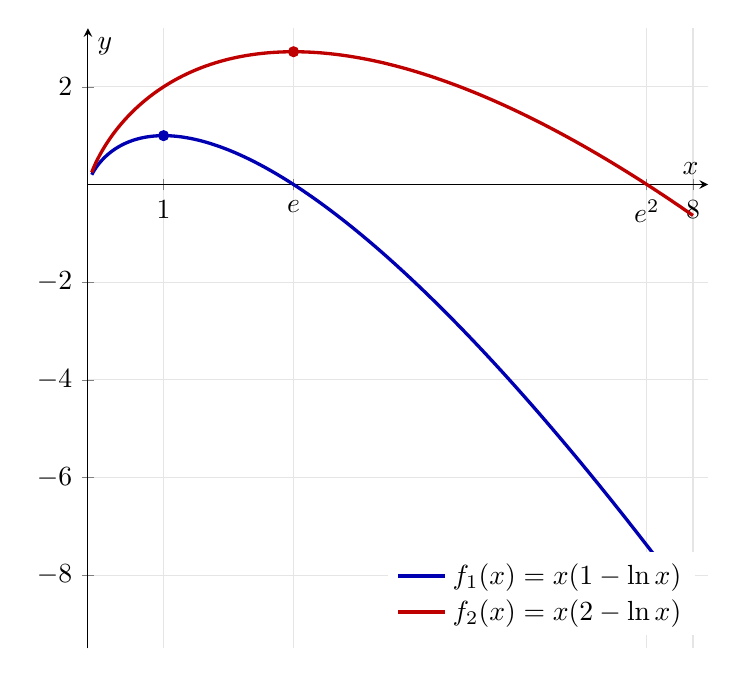
\begin{tikzpicture}
			 \begin{axis}[
			 	width=0.78\textwidth,
			 	height=0.78\textwidth,
			 	axis lines=middle,
			 	xlabel={$x$},
			 	ylabel={$y$},
			 	xmin=0, xmax=8.2,
			 	ymin=-9.5, ymax=3.2,
			 	domain=0.05:8,
			 	samples=300,
			 	grid=both,
			 	grid style={gray!20},
			 	minor grid style={gray!10},
			 	legend style={at={(0.98,0.02)},anchor=south east,fill=white,draw=none},
			 	xtick={1,2.7182818,7.3890561,8},
			 	xticklabels={$1$,$e$,$e^2$,$8$}
			 ]
			 	\addplot[very thick, blue!70!black] {x*(1-ln(x))};
			 	\addlegendentry{$f_1(x)=x(1-\ln x)$}
			 	\addplot[very thick, red!75!black] {x*(2-ln(x))};
			 	\addlegendentry{$f_2(x)=x(2-\ln x)$}
			 	\addplot[only marks, mark=*, mark size=1.8pt, blue!70!black] coordinates {(1,1)};
			 	\addplot[only marks, mark=*, mark size=1.8pt, red!75!black] coordinates {(2.7182818,2.7182818)};
			 \end{axis}
			 \end{tikzpicture}
			 \end{minipage}
			 \item $F_a(x)=\frac{x^2}{2}(a-\ln x +\frac{1}{2})$
			 \item $A=\int_0^{e} f_1(x)\,\mathrm{d}x =F(e)-F(1)=\frac{1}{4}e^2-\frac{3}{4} \approx 1.1$
			 \item \[
			 \begin{aligned}
			 A(a)&=\lim_{t\to 0}\int_t^{e^a} x(a-\ln x)\,\mathrm{d}x \\
			 &=\lim_{t\to 0}\left[\frac{ax^2}{2}+\frac{x^2}{4}-\frac{x^2}{2}\ln x\right]_{t}^{e^a} \\
			 &=\frac{1}{4}e^{2a}-\lim_{t\to 0}\left(\frac{at^2}{2}+\frac{t^2}{4}-\frac{t^2}{2}\ln t\right) \\
			 &=\frac{1}{4}e^{2a}
			 \end{aligned}
			 \]		
 		}
	\komplexloesung{}{
		\item $f_a'(x)=2a^2x-\frac{a}{x},f_a''(x)=2a^2+\frac{a}{x^2}$
		\item $T(\frac{1}{\sqrt{2a}}|\frac{a}{2}\left(1+\ln(2a)\right))$, keine Wendepunkte
		\item siehe Abbildung
		\item $f_1(x)\geq \frac{1}{2}(1+\ln 2)\approx 0.85>0$
		\item $\frac{a}{2}\left(1+\ln(2a)\right)=0\Longrightarrow a=\frac{1}{2e}$
	}
	\komplexloesung{}{
		\item $f_a'(x)=2x-\frac{a}{x}, f_a''(x)=2+\frac{a}{x^2}$
		\item $T(\sqrt{\frac{a}{2}}|\frac{a}{2}\left(1-\ln \left(\frac{a}{2}\right)\right)),f_a''(x)\neq 0 \Longrightarrow$ keine Wendepunkte
		\item \begin{minipage}[t]{\linewidth}
				\vspace{0pt}
				\centering
				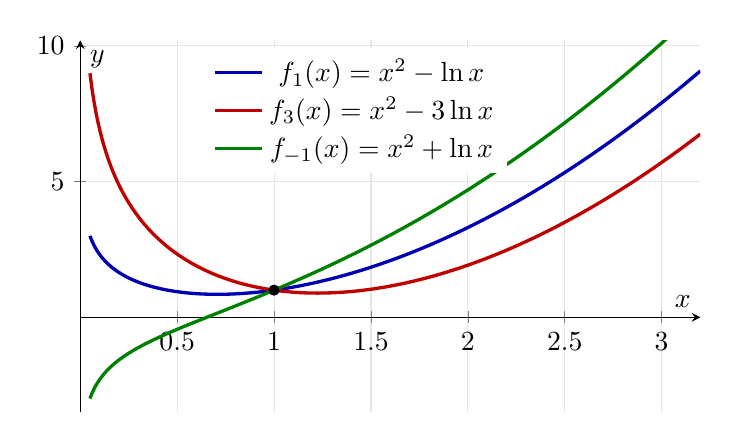
\begin{tikzpicture}
					\begin{axis}[
						width=0.78\textwidth,
						height=0.52\textwidth,
						axis lines=middle,
						xlabel={$x$},
						ylabel={$y$},
						xmin=0, xmax=3.2,
						ymin=-3.5, ymax=10.2,
						domain=0.05:3.2,
						samples=300,
						grid=both,
						grid style={gray!20},
						minor grid style={gray!10},
						legend style={at={(0.2,0.98)},anchor=north west,fill=white,draw=none}
					]
						\addplot[very thick, blue!70!black] {x^2 - ln(x)};
						\addlegendentry{$f_1(x)=x^2-\ln x$}
						\addplot[very thick, red!75!black] {x^2 - 3*ln(x)};
						\addlegendentry{$f_3(x)=x^2-3\ln x$}
						\addplot[very thick, green!50!black] {x^2 + ln(x)};
						\addlegendentry{$f_{-1}(x)=x^2+\ln x$}
						\addplot[only marks, mark=*, mark size=1.8pt, black] coordinates {(1,1)};
					\end{axis}
				\end{tikzpicture}
			\end{minipage}
		\item $\frac{a}{2}\left(1-\ln\left(\frac{a}{2}\right)\right)=0, a=2e$
		\item $\frac{a}{2}\left(1-\ln\left(\frac{a}{2}\right)\right)<0\Longrightarrow$ 2 Nullstellen, also für $1<\ln\left(\frac{a}{2}\right)$ 2 Nullstellen für $a>2e$,
		$\frac{a}{2}\left(1-\ln\left(\frac{a}{2}\right)\right)=0\Longrightarrow$ eine Nullstelle für $a=2e$, 
		$\frac{a}{2}\left(1-\ln\left(\frac{a}{2}\right)\right)>0\Longrightarrow$ keine Nullstellen für $a<2e$
		\item $F_a(x)=\frac{1}{3}x^3-ax\ln x +ax$
		\item Wendepunkte: $W\left(\sqrt{\frac{-a}{2}}\;\middle|\;-\frac{a}{2}\left(1+\ln \left(\frac{-a}{2}\right)\right)\right)$ keine Extrema, alle Graphen gehen durch $P(1|1)$. 
		Für $a_1<a_2$ gilt: $f_{a_1}<f_{a_2}$ für $x<1$,$f_{a_1}>f_{a_2}$ für $x>1$. Wegen $\lim_{x\to 0}f_a(x)=-\infty<0$ und $f_a(1)=1>0$ muss für $a<0$ eine Nullstelle existieren.
	}
	\komplexloesung{}{
		\item $f_a'(x)=2\ln (ax)\cdot\frac{1}{x}, f_a''(x)=\frac{2}{x^2}\left(1-\ln (ax)\right), f_a'''(x)=-\frac{6}{x^3}+\frac{4}{x^3}\ln (ax)$
		\item Nullstellen: $x_{1/2}=\frac{1}{a}e^{\pm\sqrt{a}}$, Extrema: $T\left(\frac{1}{a}|-a\right)$
		\item Wendepunkte: $1-\ln(ax)=0\Longrightarrow x=\frac{e}{a}, W\left(\frac{e}{a}|1-a\right)$
		\item \begin{minipage}[t]{\linewidth}
				\vspace{0pt}
				\centering
				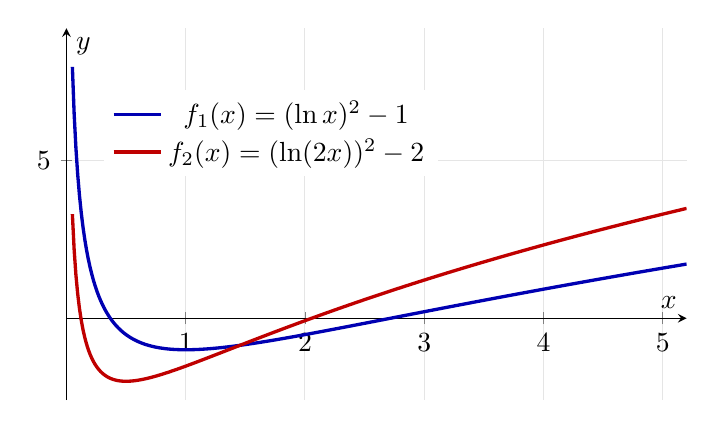
\begin{tikzpicture}
					\begin{axis}[
						width=0.78\textwidth,
						height=0.52\textwidth,
						axis lines=middle,
						xlabel={$x$},
						ylabel={$y$},
						xmin=0, xmax=5.2,
						ymin=-2.6, ymax=9.2,
						domain=0.05:5.2,
						samples=350,
						grid=both,
						grid style={gray!20},
						minor grid style={gray!10},
						legend style={at={(0.6,0.6)},anchor=south east,fill=white,draw=none}
					]
						\addplot[very thick, blue!70!black] {(ln(x))^2 - 1};
						\addlegendentry{$f_1(x)=(\ln x)^2-1$}
						\addplot[very thick, red!75!black] {(ln(2*x))^2 - 2};
						\addlegendentry{$f_2(x)=(\ln(2x))^2-2$}
					\end{axis}
				\end{tikzpicture}
			\end{minipage}
		\item $\lim_{x\to 0}f_a(x)=\infty, \lim_{x\to \infty}f_a(x)=\infty$
		\item $t(x)=\frac{2a}{e}x-1-a,a=3$
		\item Ortskurve der Extrema: $y(x)=-\frac{1}{x}$
		\item Ortskurve der Wendepunkte: $y(x)=1-\frac{e}{x}$
		\item Mit Hilfe der linearen Substitution überlegt man sich dass gilt: \newline $\int f(a\cdot x) \mathrm{d}x \overset{t=a\cdot x}{=} \frac{1}{a}\int f(t) \mathrm{d}t $
		Daher transformiert sich: $\int \ln x \ln x\mathrm{d}x$ zu $\frac{1}{a}\int \ln t \ln t\mathrm{d}t$ was durch partielle Integration gelöst werden kann. Es ergibt sich: $F_a(x)=x\left(\ln^2(ax)-2\ln ax+2-a\right)$ 
	}	
		
	\end{komplexloesungen}
\end{loesungssektion}


\end{document}
